\documentclass[usenames,dvipsnames,aspectratio=169]{beamer}

\usepackage[utf8]{inputenc}
\usepackage[T1]{fontenc}
\usepackage[magyar]{babel}
\usepackage{indentfirst}
\usepackage{listingsutf8}
\lstset{literate=
  {á}{{\'a}}1 {é}{{\'e}}1 {í}{{\'i}}1 {ó}{{\'o}}1 {ú}{{\'u}}1
  {Á}{{\'A}}1 {É}{{\'E}}1 {Í}{{\'I}}1 {Ó}{{\'O}}1 {Ú}{{\'U}}1
  {à}{{\`a}}1 {è}{{\`e}}1 {ì}{{\`i}}1 {ò}{{\`o}}1 {ù}{{\`u}}1
  {À}{{\`A}}1 {È}{{\'E}}1 {Ì}{{\`I}}1 {Ò}{{\`O}}1 {Ù}{{\`U}}1
  {ä}{{\"a}}1 {ë}{{\"e}}1 {ï}{{\"i}}1 {ö}{{\"o}}1 {ü}{{\"u}}1
  {Ä}{{\"A}}1 {Ë}{{\"E}}1 {Ï}{{\"I}}1 {Ö}{{\"O}}1 {Ü}{{\"U}}1
  {â}{{\^a}}1 {ê}{{\^e}}1 {î}{{\^i}}1 {ô}{{\^o}}1 {û}{{\^u}}1
  {Â}{{\^A}}1 {Ê}{{\^E}}1 {Î}{{\^I}}1 {Ô}{{\^O}}1 {Û}{{\^U}}1
  {œ}{{\oe}}1 {Œ}{{\OE}}1 {æ}{{\ae}}1 {Æ}{{\AE}}1 {ß}{{\ss}}1
  {ç}{{\c c}}1 {Ç}{{\c C}}1 {ø}{{\o}}1 {å}{{\r a}}1 {Å}{{\r A}}1
  {€}{{\EUR}}1 {£}{{\pounds}}1 {ő}{{\H{o}}}1
}
\lstdefinestyle{cpp}{
  language=[ISO]C++,
  showstringspaces=false,
  keywordstyle=\color{MidnightBlue}\bfseries,
  stringstyle=\color{DarkOrchid},
  commentstyle=\color{Brown},
  morecomment=[l][\color{OliveGreen}]{\#}
}
\usepackage{hyperref}
\usepackage{attachfile}
\usepackage{multirow}
% Navigációs pöttyök hozzáadása subsection nélküli fejezetekhez
\usepackage{remreset}
\makeatletter
\@removefromreset{subsection}{section}
\makeatother
\setcounter{subsection}{1}
%%%%%
\attachfilesetup{color={1.0 0.6 0.0},author={HFM},description={Kattintson duplán a minta %
megtekintéséhez!},icon=Paperclip}
\usetheme{Warsaw}
\definecolor{kiemelesszin}{rgb}{0.6,0.0,0.0}
\definecolor{kiemelesszinZ}{rgb}{0.0,0.6,0.0}
\definecolor{kiemelesszinN}{RGB}{196,127,0}
\definecolor{hivatkozasszin}{rgb}{0.0,0.0,0.75}
\newcommand{\kiemel}[1]{{\color{kiemelesszin}#1}}
\newcommand{\kiemelZ}[1]{{\color{kiemelesszinZ}#1}}
\newcommand{\kiemelN}[1]{{\color{kiemelesszinN}#1}}
\newcommand{\hiv}[1]{{\color{hivatkozasszin}#1}}
\frenchspacing
\usetheme[compress]{Berlin}

\title[Modern szoftverfejlesztési eszközök - egységtesztek]{C++ programok egységtesztelése googletest segítségével}
\subtitle{(GKxB\_INTM006)}
\author{Dr. Hatwágner F. Miklós}
\institute{Széchenyi István Egyetem, Győr}
\date{\hiv{\href{https://github.com/wajzy/GKxB\_INTM006.git}{https://github.com/wajzy/GKxB\_INTM006.git}}\\ \today}

\begin{document}

%1
\begin{frame}[plain]
  \titlepage
\end{frame}

\section{Bevezetés}

\begin{frame}
  Tesztelés célja: a hibákat megtalálni üzembe helyezés előtt
  \vfill
  Tesztelés alapelvei
  \begin{enumerate}
    \item A tesztelés bizonyos hibák jelenlétét jelezheti (ha nem jelzi, az nem jelent automatikusan hibamentességet)
    \item Nem lehetséges kimerítő teszt (a hangsúly a magas kockázatú részeken van)
    \item Korai teszt (minél hamarabb találjuk meg a hibát, annál olcsóbb javítani)
    \item Hibák csoportosulása (azokra a modulokra/bemenetekre kell tesztelni, amelyre a legvalószínűbben hibás a szoftver)
    \item Féregirtó paradoxon (a tesztesetek halmazát időnként bővíteni kell, mert ugyanazokkal a tesztekkel nem fedhetünk fel 
    több hibát)
    \item Körülmények (tesztelés alapossága függ a felhasználás helyétől, a rendelkezésre álló időtől, stb.)
    \item A hibátlan rendszer téveszméje (A megrendelő elsősorban az igényeinek megfelelő szoftvert szeretne, és csak 
    másodsorban hibamenteset; verifikáció vs. validáció)
  \end{enumerate}
\end{frame}

\begin{frame}
  Tesztelési technikák
  \begin{description}[mm]
    \item[Fekete dobozos (black-box, specifikáció alapú)] \hfill\\ A tesztelő nem látja a forrást, de a specifikációt igen, és 
hozzáfér a futtatható szoftverhez. Összehasonlítjuk a bemenetekre adott kimeneteket az elvárt kimenetekkel.
    \item[Fehér dobozos (white-box, strukturális teszt)] \hfill\\ Kész struktúrákat tesztelünk, pl.:
    \begin{itemize}
      \item kódsorok,
      \item elágazások,
      \item metódusok,
      \item osztályok,
      \item funkciók,
      \item modulok.
    \end{itemize}
    Lefedettség: a struktúra hány \%-át tudjuk tesztelni a tesztesetekkel?\\
    Egységteszt (unit test): a metódusok struktúra tesztje.
  \end{description}
\end{frame}

\begin{frame}
  A tesztelés szintjei:
  \begin{enumerate}
    \item komponensteszt (egy komponens tesztelése)
    \begin{enumerate}
      \renewcommand{\theenumii}{\alph{enumii}}
      \item egységteszt
      \item modulteszt
    \end{enumerate}
    \item integrációs teszt (kettő vagy több komponens együttműködése)
    \item rendszerteszt (minden komponens együtt)
    \item átvételi teszt (kész rendszer)
  \end{enumerate}
\end{frame}

\begin{frame}
  Kik végzik a tesztelést?
  \begin{itemize}
    \item[1-3] Fejlesztő cég
    \item[4] Felhasználók
  \end{itemize}
  Komponensteszt
  \begin{itemize}
    \item fehér dobozos teszt
    \item egységteszt
    \begin{itemize}
      \item bemenet $\to$ kimenet vizsgálata
      \item nem lehet mellékhatása
      \item regressziós teszt: módosítással elronthattunk valamit, ami eddig jó volt $\to$ megismételt egységtesztek
    \end{itemize}
    \item modulteszt
    \begin{itemize}
      \item nem funkcionális tulajdonságok: sebesség, memóriaszivárgás (memory leak), szűk keresztmetszetek (bottleneck)
    \end{itemize}
  \end{itemize}
\end{frame}

\begin{frame}
  Integrációs teszt
  \begin{itemize}
    \item Komponensek közötti interfészek ellenőrzése, pl.
    \begin{itemize}
      \item komponens - komponens (egy rendszer komponenseinek együttműködése)
      \item rendszer - rendszer (pl. OS és a fejlesztett rendszer között)
    \end{itemize}
    \item Jellemző hibaokok: komponenseket eltérő csapatok fejlesztik, elégtelen kommunikáció
    \item Kockázatok csökkentése: mielőbbi integrációs tesztekkel
  \end{itemize}
\end{frame}

\begin{frame}
  Rendszerteszt: a termék megfelel-e a
  \begin{itemize}
    \item követelmény specifikációnak,
    \item funkcionális specifikációnak,
    \item rendszertervnek.
  \end{itemize}
  Gyakran fekete dobozos, külső cég végzi (elfogulatlanság)\\
  Leendő futtatási környezet imitációja
\end{frame}

\begin{frame}
  Átvételi teszt, fajtái:
  \begin{itemize}
    \item alfa: kész termék tesztelése a fejlesztőnél, de nem általa (pl. segédprogramok)
    \item béta: szűk végfelhasználói csoport
    \item felhasználói átvételi teszt: minden felhasználó használja, de nem éles termelésben. Jellemző a környezetfüggő hibák 
    megjelenése (pl. sebesség)
    \item üzemeltetői átvételi teszt: rendszergazdák végzik, biztonsági mentés, helyreállítás, stb. helyesen működnek-e
  \end{itemize}
\end{frame}


\section{C++}

\begin{frame}
 Rengeteg C++ egységteszt keretrendszerből lehet választani:
 \begin{itemize}
   \item \hiv{\href{https://en.wikipedia.org/wiki/List\_of\_unit\_testing\_frameworks\#C++}{Wiki oldal}}
   \item \hiv{\href{http://gamesfromwithin.com/exploring-the-c-unit-testing-framework-jungle}%
     {Exploring the C++ Unit Testing Framework Jungle}}
   \item \hiv{\href{https://accu.org/index.php/journals/1326}{C++ Unit Test Frameworks}}
 \end{itemize}
 \vfill
 Részletesen megvizsgáljuk: googletest
\end{frame}

\section{googletest}

\subsection{Az első teszprogram elkészítése}

\begin{frame}
  A googletest főbb tulajdonságai
  \begin{itemize}
    \item platformfüggetlen (Linux, Windows, Mac)
    \item független és megismételhető tesztek
    \item struktúrálható tesztek (teszt program $\to$ teszt csomag $\to$ teszteset)
    \item informatív
    \item leveszi a tesztelés technikai részének terhét a tesztelőről
    \item gyors (megosztott erőforrások)
    \item könnyen tanulható (xUnit architektúra)
  \end{itemize}
\end{frame}

\begin{frame}
  Telepítés (Ubuntu 18.04 LTS)
  \begin{description}[m]
    \item[\texttt{sudo apt install libgtest-dev}] \hfill \\ Teszt keretrendszer forrásainak beszerzése.
    \item[\texttt{sudo apt install cmake}] \hfill \\ Ezzel végezzük a forráskódok automatizált fordítását.
    \item[\texttt{cd /usr/src/gtest}] \hfill \\ Ebben a mappában találhatóak a források.
    \item[\texttt{sudo cmake CMakeLists.txt}] \hfill \\ Összeállító (build) környezet előkészítése.
    \item[\texttt{sudo make}] \hfill \\ Összeállítás indítása.
  \end{description}
\end{frame}

\begin{frame}
  \begin{description}[m]
    \item[\texttt{sudo ln -st /usr/lib/ /usr/src/gtest/libgtest.a}]
    \item[\texttt{sudo ln -st /usr/lib/ /usr/src/gtest/libgtest\_main.a}] \hfill \\ Szimbolikus hivatkozások létrehozása.
  \end{description}
  \vfill
  Feladat
  \begin{itemize}
    \item[] Készítsünk mátrixműveleteket megvalósító osztályt, ami elsőként egy mátrixszorzást valósít meg.
    \item[] Az $A[a_{i,j}]_{m\times{n}}$ és $B[b_{i,j}]_{n\times{p}}$mátrixok
szorzatán azt a $C[c_{i,j}]_{m\times{p}}$ mátrixot értjük, amelyre $c_{i,j} =
a_{i,1}\cdot{b}_{1,j} + a_{i,2}\cdot{b}_{2,j} + \dots + a_{i,n}\cdot{b}_{n,j} =
\sum_{k=1}^{n}a_{i,k}\cdot{b}_{k,j}$ 
  \end{itemize}
\end{frame}

\begin{frame}
  \begin{exampleblock}{\textattachfile{01/matrix01.h}{01/matrix01.h}}
    \footnotesize
    \lstinputlisting[style=cpp,linerange={1-13},numbers=left,firstnumber=1]{01/matrix01.h}
  \end{exampleblock}
\end{frame}

\begin{frame}
  \begin{exampleblock}{\textattachfile{01/matrix01.h}{01/matrix01.h}}
    \lstinputlisting[style=cpp,linerange={14-19},numbers=left,firstnumber=14]{01/matrix01.h}
  \end{exampleblock}
\end{frame}

\begin{frame}
  \begin{exampleblock}{\textattachfile{01/matrix01.h}{01/matrix01.h}}
    \lstinputlisting[style=cpp,linerange={21-29},numbers=left,firstnumber=21]{01/matrix01.h}
  \end{exampleblock}
\end{frame}

\begin{frame}
  \begin{exampleblock}{\textattachfile{01/matrix01.h}{01/matrix01.h}}
    \footnotesize
    \lstinputlisting[style=cpp,linerange={31-43},numbers=left,firstnumber=31]{01/matrix01.h}
  \end{exampleblock}
\end{frame}

\begin{frame}
  \begin{exampleblock}{\textattachfile{01/matrix01.h}{01/matrix01.h}}
    \small
    \lstinputlisting[style=cpp,linerange={45-56},numbers=left,firstnumber=45]{01/matrix01.h}
  \end{exampleblock}
\end{frame}

\begin{frame}
  \begin{exampleblock}{\textattachfile{01/example01.cpp}{01/example01.cpp}}
    \small
    \lstinputlisting[style=cpp,linerange={1-13},numbers=left,firstnumber=1]{01/example01.cpp}
  \end{exampleblock}
\end{frame}

\begin{frame}[fragile]
  \begin{exampleblock}{\textattachfile{01/example01.cpp}{01/example01.cpp}}
    \small
    \lstinputlisting[style=cpp,linerange={14-21},numbers=left,firstnumber=14]{01/example01.cpp}
  \end{exampleblock}
  \begin{block}{Kimenet}
    \begin{verbatim}
50      50      50
90      90      90
130     130     130
\end{verbatim}
  \end{block}
\end{frame}

\begin{frame}
  Készítsünk az \texttt{example01.cpp} alapján googletest alapú tesztprogramot!
  \begin{exampleblock}{\textattachfile{01/matrix01test.cpp}{01/matrix01test.cpp}}
    \footnotesize
    \lstinputlisting[style=cpp,linerange={1-12},numbers=left,firstnumber=1]{01/matrix01test.cpp}
  \end{exampleblock}
\end{frame}

\begin{frame}
  \begin{exampleblock}{\textattachfile{01/matrix01test.cpp}{01/matrix01test.cpp}}
    \lstinputlisting[style=cpp,linerange={13-20},numbers=left,firstnumber=13]{01/matrix01test.cpp}
  \end{exampleblock}
\end{frame}

\begin{frame}
  \begin{exampleblock}{\textattachfile{01/matrix01test.cpp}{01/matrix01test.cpp}}
    \footnotesize
    \lstinputlisting[style=cpp,linerange={21-33},numbers=left,firstnumber=21]{01/matrix01test.cpp}
  \end{exampleblock}
\end{frame}

\begin{frame}
  \begin{exampleblock}{\textattachfile{01/CMakeLists.txt}{01/CMakeLists.txt}}
    \footnotesize
    \lstinputlisting[style=cpp,linerange={1-1},numbers=left,firstnumber=1]{01/CMakeLists.txt}
    \lstinputlisting[style=cpp,linerange={14-21},numbers=left,firstnumber=14]{01/CMakeLists.txt}
  \end{exampleblock}
\end{frame}

\begin{frame}[fragile]
  \begin{description}[m]
    \footnotesize
    \item[\texttt{cmake CMakeLists.txt}] \hfill \\ Összeállító (build) környezet beállítása.
    \item[\texttt{make}] \hfill \\ Összeállítás indítása.
    \item[\texttt{./runTests}] \hfill \\ Tesztprogram indítása.
  \end{description}
  \begin{block}{Kimenet}
    \scriptsize
    \begin{verbatim}
[==========] Running 1 test from 1 test case.
[----------] Global test environment set-up.
[----------] 1 test from MulTest
[ RUN      ] MulTest.meaningful
[       OK ] MulTest.meaningful (0 ms)
[----------] 1 test from MulTest (0 ms total)

[----------] Global test environment tear-down
[==========] 1 test from 1 test case ran. (0 ms total)
[  PASSED  ] 1 test.
\end{verbatim}
  \end{block}
\end{frame}

\begin{frame}
  \begin{description}[m]
    \item[Teszteset (test case)] \hfill \\ "A set of preconditions, inputs, actions (where applicable), %
      expected results and postconditions, developed based on test conditions."\\
      (meaningful, ld. \texttt{matrix01test.ccp} 5. sor)
    \item[Tesztkészlet (test suite)] \hfill \\ "A set of test cases or test procedures to be executed in a specific test cycle."\\
      (MulTest, ld. \texttt{matrix01test.ccp} 5. sor)
    \item[Tesztprogram (test program)] \hfill \\ Egy vagy több tesztkészletet foglal magába.
  \end{description}
  Sajnos a googletest nevezéktana következetlen: \medskip\\
  \begin{tabular}{ll}
    \textbf{googletest} & \textbf{ISTQB}\\\hline
    teszt (test) & teszteset\\
    teszteset (test case) & tesztkészlet
  \end{tabular}
\end{frame}

\begin{frame}
  \begin{description}[m]
    \item[Assertion ($\approx$ állítás, követelés)] Ellenőrizzük valamely elvárásunk teljesülését $\to$ siker (success), %
      nem végzetes hiba (nonfatal failure), végzetes hiba (fatal failure).\\
      Makrók:
      \begin{description}[m]
        \item[\texttt{EXPECT\_*}] nem végzetes hibát generál, ajánlott (több hiba jelezhető egyszerre)
        \item[\texttt{ASSERT\_*}] végzetes hibát generál, azonnal leállítja a tesztesetet (nincs értelme a folytatásnak; pl. ha két mátrix nem azonos méretű, nincs értelme az elemeiket összehasonlítgatni). \kiemel{Erőforrások felszabadítása, takarítás is elmarad!}
      \end{description}
  \end{description}
\end{frame}

\begin{frame}
  Rontsuk el a kódot! (,,Elfelejtjük'' összegezni a szorzatokat.)
  \begin{exampleblock}{\textattachfile{02/matrix02.h}{02/matrix02.h} %
    (\textattachfile{02/matrix02test.cpp}{02/matrix02test.cpp}, %
    \textattachfile{02/CMakeLists.txt}{02/CMakeLists.txt})}
    \lstinputlisting[style=cpp,linerange={45-51},numbers=left,firstnumber=45]{02/matrix02.h}
  \end{exampleblock}
\end{frame}

\begin{frame}[fragile]
  \begin{block}{Kimenet}
    \footnotesize
    \begin{verbatim}
[==========] Running 1 test from 1 test case.
[----------] Global test environment set-up.
[----------] 1 test from MulTest
[ RUN      ] MulTest.meaningful
/home/wajzy/Dokumentumok/gknb_intm006/GKxB_INTM006/02/matrix02test.cpp:25: Failure
      Expected: expected[row][col]
      Which is: 50
To be equal to: multiplied.get(row, col)
      Which is: 0
...
\end{verbatim}
  \end{block}
\end{frame}

\begin{frame}[fragile]
  \footnotesize
  \begin{block}{Kimenet}
    \begin{verbatim}
...
/home/wajzy/Dokumentumok/gknb_intm006/GKxB_INTM006/02/matrix02test.cpp:25: Failure
      Expected: expected[row][col]
      Which is: 130
To be equal to: multiplied.get(row, col)
      Which is: 0
[  FAILED  ] MulTest.meaningful (1 ms)
[----------] 1 test from MulTest (1 ms total)

[----------] Global test environment tear-down
[==========] 1 test from 1 test case ran. (1 ms total)
[  PASSED  ] 0 tests.
[  FAILED  ] 1 test, listed below:
[  FAILED  ] MulTest.meaningful

 1 FAILED TEST
\end{verbatim}
  \end{block}
\end{frame}

\begin{frame}
  Most rontsuk el másképp a kódot! (Túl nagy lesz az eredmény mátrix.)
  \begin{exampleblock}{\textattachfile{03/matrix03.h}{03/matrix03.h} %
    (\textattachfile{03/CMakeLists.txt}{03/CMakeLists.txt})}
    \lstinputlisting[style=cpp,linerange={40-44},numbers=left,firstnumber=40]{03/matrix03.h}
  \end{exampleblock}
\end{frame}

\begin{frame}
  \begin{exampleblock}{\textattachfile{03/matrix03test.cpp}{03/matrix03test.cpp}}
    \footnotesize
    \lstinputlisting[style=cpp,linerange={21-33},numbers=left,firstnumber=21]{03/matrix03test.cpp}
  \end{exampleblock}
\end{frame}

\begin{frame}[fragile]
  \begin{block}{Kimenet}
    \tiny
    \begin{verbatim}
[==========] Running 1 test from 1 test case.
[----------] Global test environment set-up.
[----------] 1 test from MulTest
[ RUN      ] MulTest.meaningful
/home/wajzy/Dokumentumok/gknb_intm006/GKxB_INTM006/03/matrix03test.cpp:21: Failure
      Expected: expected.size()
      Which is: 3
To be equal to: multiplied.getRowCount()
      Which is: 6
A sorok szama elter! Elvart: 3, kapott: 6
[  FAILED  ] MulTest.meaningful (0 ms)
[----------] 1 test from MulTest (0 ms total)

[----------] Global test environment tear-down
[==========] 1 test from 1 test case ran. (0 ms total)
[  PASSED  ] 0 tests.
[  FAILED  ] 1 test, listed below:
[  FAILED  ] MulTest.meaningful

 1 FAILED TEST
\end{verbatim}
  \end{block}
  \begin{itemize}
    \item Az \texttt{ASSERT\_EQ} leállította a tesztesetet.
    \item Testreszabott hibaüzeneteket jelenítettünk meg.
  \end{itemize}
\end{frame}

\begin{frame}
  \begin{center}
    Elemi követelmények
    \medskip\\
    \begin{tabular}{lll}
      \textbf{Végzetes hibákhoz} & \textbf{Nem végzetes hibákhoz} & \textbf{Követelmény}\\ \hline
      ASSERT\_TRUE(\emph{feltétel}) & EXPECT\_TRUE(\emph{feltétel}) & \emph{feltétel} igaz értékű\\
      ASSERT\_FALSE(\emph{feltétel}) & EXPECT\_FALSE(\emph{feltétel}) & \emph{feltétel} hamis értékű
    \end{tabular}
  \end{center}
\end{frame}

\begin{frame}
  \begin{center}
    Relációs követelmények
    \medskip\\
    \begin{tabular}{lll}
      \textbf{Végzetes hibákhoz} & \textbf{Nem végzetes hibákhoz} & \textbf{Követelmény}\\ \hline
      ASSERT\_EQ(\emph{val1}, \emph{val2}); & EXPECT\_EQ(\emph{val1}, \emph{val2}); & \emph{val1} == \emph{val2}\\
      ASSERT\_NE(\emph{val1}, \emph{val2}); & EXPECT\_NE(\emph{val1}, \emph{val2}); & \emph{val1} != \emph{val2}\\
      ASSERT\_LT(\emph{val1}, \emph{val2}); & EXPECT\_LT(\emph{val1}, \emph{val2}); & \emph{val1} < \emph{val2}\\
      ASSERT\_LE(\emph{val1}, \emph{val2}); & EXPECT\_LE(\emph{val1}, \emph{val2}); & \emph{val1} <= \emph{val2}\\
      ASSERT\_GT(\emph{val1}, \emph{val2}); & EXPECT\_GT(\emph{val1}, \emph{val2}); & \emph{val1} > \emph{val2}\\
      ASSERT\_GE(\emph{val1}, \emph{val2}); & EXPECT\_GE(\emph{val1}, \emph{val2}); & \emph{val1} >= \emph{val2}
    \end{tabular}
  \end{center}
\end{frame}

\begin{frame}
  Megjegyzések
  \begin{itemize}
    \item A feltüntetett operátoroknak definiáltnak kell lenniük \emph{val1} és \emph{val2} között. Lehetőségeink:
    \begin{enumerate}
      \item Felültöltjük az operátorokat.
      \item Az \{ASSERT,EXPECT\}\_\{TRUE,FALSE\} makrókat használjuk, de ezek nem írják a kimenetre az elvárt/kapott 
értékeket.
    \end{enumerate}
    \item A paraméterek egyszer lesznek kiértékelve, de nem definiált sorrendben (mellékhatások).
    \item Az \{ASSERT,EXPECT\}\_EQ makrók mutatók esetén a címeket hasonlítja össze, nem az ott lévő tartalmat! C-stílusú 
karakterláncok kezeléséhez külön makrók léteznek. (\texttt{string} objektumokkal nincs gond.)
    \item C++11 szabványnak megfelelő fordító esetén \texttt{NULL} helyett \texttt{nullptr}-t használjunk 
(utóbbi nem konvertálható implicit módon \texttt{int}-té)!
    \item Lebegőpontos számok összehasonlításakor kerekítési hibák adódhatnak.
  \end{itemize}
\end{frame}


\subsection{Lebegőpontos számok kezelése}

\begin{frame}
  Készítsünk lebegőpontos számokból álló mátrixokat, majd teszteljük a szorzást ismét!
  \begin{exampleblock}{\textattachfile{04/matrix04test.cpp}{04/matrix04test.cpp} %
    (\textattachfile{04/matrix04.h}{04/matrix04.h}, %
     \textattachfile{04/CMakeLists.txt}{04/CMakeLists.txt})}
    \small
    \lstinputlisting[style=cpp,linerange={31-41},numbers=left,firstnumber=31]{04/matrix04test.cpp}
  \end{exampleblock}
\end{frame}

\begin{frame}
  \begin{exampleblock}{\textattachfile{04/matrix04test.cpp}{04/matrix04test.cpp}}
    \small
    \lstinputlisting[style=cpp,linerange={42-52},numbers=left,firstnumber=42]{04/matrix04test.cpp}
  \end{exampleblock}
\end{frame}

\begin{frame}[fragile]
  \begin{block}{Kimenet}
    \scriptsize
    \begin{verbatim}
...
[ RUN      ] MulTest.rounding
/home/wajzy/Dokumentumok/gknb_intm006/GKxB_INTM006/04/matrix04test.cpp:49: Failure
Value of: multiplied.get(row, col)
  Actual: 1.41421
Expected: expected[row][col]
Which is: 1.41421
...
/home/wajzy/Dokumentumok/gknb_intm006/GKxB_INTM006/04/matrix04test.cpp:49: Failure
Value of: multiplied.get(row, col)
  Actual: 0.333333
Expected: expected[row][col]
Which is: 0.333333
[  FAILED  ] MulTest.rounding (0 ms)
...
\end{verbatim}
  \end{block}
  A kerekítési hibák érzékelhetetlenek a kimeneten és a teszt sikertelen.
\end{frame}

\begin{frame}
  Próbálkozzunk a beépített, lebegőpontos számokat összehasonlító makrókkal!
  \begin{exampleblock}{\textattachfile{05/matrix05test.cpp}{05/matrix05test.cpp} %
    (\textattachfile{05/matrix05.h}{05/matrix05.h}, %
     \textattachfile{05/CMakeLists.txt}{05/CMakeLists.txt})}
    \footnotesize
    \lstinputlisting[style=cpp,linerange={47-52},numbers=left,firstnumber=47]{05/matrix05test.cpp}
  \end{exampleblock}
\end{frame}

\begin{frame}[fragile]
  \begin{block}{Kimenet}
    \scriptsize
    \begin{verbatim}
...
[ RUN      ] MulTest.rounding
/home/wajzy/Dokumentumok/gknb_intm006/GKxB_INTM006/05/matrix05test.cpp:50: Failure
Value of: multiplied.get(row, col)
  Actual: 1.4142135623730951
Expected: expected[row][col]
Which is: 1.414213562
...
/home/wajzy/Dokumentumok/gknb_intm006/GKxB_INTM006/05/matrix05test.cpp:50: Failure
Value of: multiplied.get(row, col)
  Actual: 0.33333333333333331
Expected: expected[row][col]
Which is: 0.33333333300000001
[  FAILED  ] MulTest.rounding (0 ms)
...
\end{verbatim}
  \end{block}
  Most már látszik, hogy az értékek közötti különbség nagyobb, mint %
  \hiv{\href{https://randomascii.wordpress.com/2012/02/25/comparing-floating-point-numbers-2012-edition/}{4 ULP}} %
  (Units in the Last Place), ezért tekinti őket a teszt különbözőnek.
\end{frame}

\begin{frame}
  Növeljük meg a számok közötti legnagyobb megengedett eltérést!
  \begin{exampleblock}{\textattachfile{06/matrix06test.cpp}{06/matrix06test.cpp} %
    (\textattachfile{06/matrix06.h}{06/matrix06.h}, %
     \textattachfile{06/CMakeLists.txt}{06/CMakeLists.txt})}
    \footnotesize
    \lstinputlisting[style=cpp,linerange={47-53},numbers=left,firstnumber=47]{06/matrix06test.cpp}
  \end{exampleblock}
\end{frame}

\begin{frame}[fragile]
  \begin{block}{Kimenet}
    \scriptsize
    \begin{verbatim}
[==========] Running 2 tests from 1 test case.
[----------] Global test environment set-up.
[----------] 2 tests from MulTest
[ RUN      ] MulTest.meaningful
[       OK ] MulTest.meaningful (0 ms)
[ RUN      ] MulTest.rounding
[       OK ] MulTest.rounding (0 ms)
[----------] 2 tests from MulTest (1 ms total)

[----------] Global test environment tear-down
[==========] 2 tests from 1 test case ran. (1 ms total)
[  PASSED  ] 2 tests.
\end{verbatim}
  \end{block}
\end{frame}

\begin{frame}
  \begin{center}
    Lebegőpontos számokkal szemben támasztható követelmények
    \medskip\\
    \resizebox{\textwidth}{!}{
    \begin{tabular}{llp{0.3\textwidth}}
      \textbf{Végzetes hibákhoz} & \textbf{Nem végzetes hibákhoz} & \textbf{Követelmény}\\ \hline
      ASSERT\_FLOAT\_EQ(\emph{val1}, \emph{val2}); & EXPECT\_FLOAT\_EQ(\emph{val1}, \emph{val2}); & \emph{float} típusú 
értékek 4 ULP-n belül\\
      ASSERT\_DOUBLE\_EQ(\emph{val1}, \emph{val2}); & EXPECT\_DOUBLE\_EQ(\emph{val1}, \emph{val2}); & \emph{double} típusú 
értékek 4 ULP-n belül\\
      ASSERT\_NEAR(\emph{val1}, \emph{val2}, \emph{abs\_error}); & EXPECT\_NEAR(\emph{val1}, \emph{val2}, \emph{abs\_error}); & 
a két érték különbségének abszolút értéke nem nagyobb \emph{abs\_error}-nál\\
    \end{tabular}
    }
  \end{center}
\end{frame}


\subsection{Operátor felültöltés}

\begin{frame}
  Próbáljuk meg a mátrixok elemenkénti összehasonlítása helyett a teljes mátrixokat összehasonlítani!
  \begin{exampleblock}{\textattachfile{07/matrix07test.cpp}{07/matrix07test.cpp} %
    (\textattachfile{07/matrix07.h}{07/matrix07.h}, %
     \textattachfile{07/CMakeLists.txt}{07/CMakeLists.txt})}
    \scriptsize
    \lstinputlisting[style=cpp,linerange={31-43},numbers=left,firstnumber=31]{07/matrix07test.cpp}
  \end{exampleblock}
\end{frame}

\begin{frame}
  \begin{exampleblock}{\textattachfile{07/matrix07test.cpp}{07/matrix07test.cpp}}
    \lstinputlisting[style=cpp,linerange={44-51},numbers=left,firstnumber=44]{07/matrix07test.cpp}
  \end{exampleblock}
\end{frame}

\begin{frame}[fragile]
  \begin{block}{Kimenet}
    \footnotesize
    \begin{verbatim}
wajzy@wajzy-notebook:~/Dokumentumok/gknb_intm006/GKxB_INTM006/07$ make
...
/home/wajzy/Dokumentumok/gknb_intm006/GKxB_INTM006/07/matrix07test.cpp:50:3: 
  required from here
/usr/include/gtest/gtest.h:1325:16: error: no match for ‘operator==’ (operand 
  types are ‘const szeMatrix::Matrix<double>’ and 
‘const szeMatrix::Matrix<double>’)
   if (expected == actual) {
                ^
...
\end{verbatim}
  \end{block}
  \vfill
  Probléma: az 50. sor \texttt{ASSERT\_EQ(mexp, multiplied);} utasítása feltételezi az == operátor felültöltését a 
\texttt{Matrix} osztályhoz.
\end{frame}

\begin{frame}
  \begin{exampleblock}{\textattachfile{08/matrix08.h}{08/matrix08.h} %
    (\textattachfile{08/matrix08test.cpp}{08/matrix08test.cpp}, %
     \textattachfile{08/CMakeLists.txt}{08/CMakeLists.txt})}
    \footnotesize
    \lstinputlisting[style=cpp,linerange={5-6},numbers=left,firstnumber=5]{08/matrix08.h}
    \lstinputlisting[style=cpp,linerange={10-10},numbers=left,firstnumber=10]{08/matrix08.h}
    \lstinputlisting[style=cpp,linerange={19-21},numbers=left,firstnumber=19]{08/matrix08.h}
    \lstinputlisting[style=cpp,linerange={58-61},numbers=left,firstnumber=58]{08/matrix08.h}
  \end{exampleblock}
\end{frame}

\begin{frame}[fragile]
  \begin{block}{Kimenet}
    \scriptsize
    \begin{verbatim}
wajzy@wajzy-notebook:~/Dokumentumok/gknb_intm006/GKxB_INTM006/08$ make
[100%] Built target runTests
wajzy@wajzy-notebook:~/Dokumentumok/gknb_intm006/GKxB_INTM006/08$ ./runTests 
[==========] Running 3 tests from 1 test case.
[----------] Global test environment set-up.
[----------] 3 tests from MulTest
[ RUN      ] MulTest.meaningful
[       OK ] MulTest.meaningful (0 ms)
[ RUN      ] MulTest.equality
[       OK ] MulTest.equality (1 ms)
[ RUN      ] MulTest.rounding
[       OK ] MulTest.rounding (0 ms)
[----------] 3 tests from MulTest (1 ms total)

[----------] Global test environment tear-down
[==========] 3 tests from 1 test case ran. (1 ms total)
[  PASSED  ] 3 tests.
\end{verbatim}
  \end{block}
\end{frame}


\subsection{Kimenet és karakterláncok kezelése}

\begin{frame}
  Teszteljük le a \texttt{print()} tagfüggvény kimenetét!
  \vfill
  \begin{tabular}{ll}
    \textbf{Függvény} & \textbf{Funkció}\\ \hline
    \texttt{CaptureStdout()} & Megkezdi az \texttt{stdout}-ra írt tartalom rögzítését\\
    \texttt{GetCapturedStdout()} & Lekérdezi a rögzített tartalmat és leállítja a rögzítést\\
    \texttt{CaptureStderr()} & Megkezdi az \texttt{stderr}-re írt tartalom rögzítését\\
    \texttt{GetCapturedStderr()} & Lekérdezi a rögzített tartalmat és leállítja a rögzítést\\
  \end{tabular}
  \vfill
  Belső tagfüggvények, használatuk \kiemel{nem javasolt} (\hiv{\href{%
https://chromium.googlesource.com/external/github.com/google/googletest/+/HEAD/googletest/include/gtest/internal/gtest-port.h}%
{googletest forráskód}}).
\end{frame}

\begin{frame}
  \begin{exampleblock}{\textattachfile{09/matrix09test.cpp}{09/matrix09.cpp} %
    (\textattachfile{09/matrix09.h}{09/matrix09.h}, %
     \textattachfile{09/CMakeLists.txt}{09/CMakeLists.txt})}
    \small
    \lstinputlisting[style=cpp,linerange={76-85},numbers=left,firstnumber=76]{09/matrix09test.cpp}
  \end{exampleblock}
\end{frame}

\begin{frame}[fragile]
  \begin{block}{Kimenet}
    \footnotesize
    \begin{verbatim}
...
[ RUN      ] MulTest.print
/home/wajzy/Dokumentumok/gknb_intm006/GKxB_INTM006/09/matrix09test.cpp:84: Failure
Value of: output.c_str()
  Actual: 0x1bb1f28
Expected: expected
Which is: 0x475e6a
[  FAILED  ] MulTest.print (0 ms)
...
\end{verbatim}
  \end{block}
  \vfill
  Probléma: a C-stílusú karakterláncok \kiemel{címeit} hasonlítja össze, nem az ott lévő tartalmat!
\end{frame}

\begin{frame}
  \begin{center}
    C-stílusú karakterláncokkal szemben támasztható követelmények
    \medskip\\
    \resizebox{\textwidth}{!}{
    \begin{tabular}{llp{0.3\textwidth}}
      \textbf{Végzetes hibákhoz} & \textbf{Nem végzetes hibákhoz} & \textbf{Követelmény}\\ \hline
      ASSERT\_STREQ(\emph{str1}, \emph{str2}); & EXPECT\_STREQ(\emph{str1}, \emph{str2}); & A két C-stílusú karakterlánc 
tartalma azonos\\
      ASSERT\_STRNE(\emph{str1}, \emph{str2}); & EXPECT\_STRNE(\emph{str1}, \emph{str2}); & A két C-stílusú karakterlánc 
tartalma eltérő\\
      ASSERT\_STRCASEEQ(\emph{str1}, \emph{str2}); & EXPECT\_STRCASEEQ(\emph{str1}, \emph{str2}); & A két C-stílusú 
karakterlánc tartalma a kis- és nagybetűk eltérésétől eltekintve azonos\\
      ASSERT\_STRCASENE(\emph{str1}, \emph{str2}); & EXPECT\_STRCASENE(\emph{str1}, \emph{str2}); & A két C-stílusú 
karakterlánc tartalma a kis- és nagybetűk eltérését figyelmen kívül hagyva is eltérő\\
    \end{tabular}
    }
  \end{center}
\end{frame}

\begin{frame}
  Javítsuk a tesztesetet és készítsünk további, hasonló tagfüggvényeket (tesztekkel)!
  \begin{exampleblock}{\textattachfile{10/matrix10test.cpp}{10/matrix10test.cpp} %
    (\textattachfile{10/CMakeLists.txt}{10/CMakeLists.txt})}
    \small
    \lstinputlisting[style=cpp,linerange={76-86},numbers=left,firstnumber=76]{10/matrix10test.cpp}
  \end{exampleblock}
\end{frame}

\begin{frame}
  \begin{exampleblock}{\textattachfile{10/matrix10.h}{10/matrix10.h}}
    \lstinputlisting[style=cpp,linerange={3-3},numbers=left,firstnumber=3]{10/matrix10.h}
    \lstinputlisting[style=cpp,linerange={7-7},numbers=left,firstnumber=7]{10/matrix10.h}
    \lstinputlisting[style=cpp,linerange={11-11},numbers=left,firstnumber=11]{10/matrix10.h}
    \lstinputlisting[style=cpp,linerange={16-18},numbers=left,firstnumber=16]{10/matrix10.h}
    \lstinputlisting[style=cpp,linerange={24-24},numbers=left,firstnumber=24]{10/matrix10.h}
  \end{exampleblock}
\end{frame}

\begin{frame}
  \begin{exampleblock}{\textattachfile{10/matrix10.h}{10/matrix10.h}}
    \scriptsize
    \lstinputlisting[style=cpp,linerange={36-51},numbers=left,firstnumber=36]{10/matrix10.h}
  \end{exampleblock}
\end{frame}

\begin{frame}
  \begin{exampleblock}{\textattachfile{10/matrix10test.cpp}{10/matrix10test.cpp}}
    \scriptsize
    \lstinputlisting[style=cpp,linerange={88-102},numbers=left,firstnumber=88]{10/matrix10test.cpp}
  \end{exampleblock}
\end{frame}


\subsection{Fixtures}

\begin{frame}
  Vegyük észre, hogy a tesztünkben egyre többször ismétlődnek részek:
  \begin{exampleblock}{\textattachfile{10/matrix10test.cpp}{10/matrix10test.cpp}}
    \tiny
    \lstinputlisting[style=cpp,linerange={76-80},numbers=left,firstnumber=76]{10/matrix10test.cpp}
    \lstinputlisting[style=cpp,linerange={88-92},numbers=left,firstnumber=88]{10/matrix10test.cpp}
    \lstinputlisting[style=cpp,linerange={96-100},numbers=left,firstnumber=96]{10/matrix10test.cpp}
  \end{exampleblock}
\end{frame}

\newcounter{fixtures}

\begin{frame}
  Megoldás: teszt \kiemel{fixture}-ök ($\approx$alkatrész) használata
  \begin{enumerate}
    \item Származtassunk le egy osztályt a \texttt{::testing::Test}-ből! Ha az \texttt{Osztaly}-t szeretnénk tesztelni, legyen 
a neve \texttt{OsztalyTest}!
    \item Deklaráljuk a többször használt tagokat! Legyenek védettek, hogy a leszármazottakból is használhatók legyenek!
    \item A tagokat inicializáljuk az alapértelmezett konstruktorban vagy a (felüldefiniált) \texttt{SetUp()} tagfüggvényben!
    \item Ha szükséges, készítsünk destruktort vagy (felüldefiniált) \texttt{TearDown()} tagfüggvényt az 
erőforrások felszabadítására!
    \item Ha szükséges, írjunk függvényeket, amiket több teszteset is hívhat!
    \setcounter{fixtures}{\theenumi}
  \end{enumerate}
\end{frame}

\begin{frame}
  \begin{enumerate}
    \setcounter{enumi}{\thefixtures}
    \item A tesztesetek definiálásakor a \texttt{TEST} helyett használjuk a \texttt{TEST\_F} makrót!
    \item A tesztkészlet neve egyezzen meg a fixture osztály nevével (\texttt{OsztalyTest})!
  \end{enumerate}
  \vfill
  Megjegyzések
  \begin{itemize}
    \item Az osztálynak már a tesztesetek makrói előtt definiáltnak kell lennie.
    \item Könnyű elgépelni a \texttt{SetUp()} és \texttt{TearDown()} függvények neveit, használjuk az \texttt{override} 
kulcsszót (C++11)!
    \item Minden egyes tesztesethez új példány készül a fixture-ből (nem ,,interferálnak'' a tesztesetek), majd:\\ 
alapértelmezett konstruktor $\to$ \texttt{SetUp()} $\to$ \texttt{TEST\_F} $\to$ \texttt{TearDown()} $\to$ destruktor.
  \end{itemize}
\end{frame}

\begin{frame}
  Mikor és miért érdemes konstruktort/destruktort használni?
  \begin{itemize}
    \item A \texttt{const} minősítővel ellátott tagváltozó csak a konstruktort követő inicializátor listával inicializálható. Jó ötlet
    a véletlen módosítások meggátolására.
    \item Ha a fixture osztályból származtatunk, az ős(ök) konstruktorának/destruktorának hívása mindenképpen végbemegy a megfelelő sorrendben. A \texttt{SetUp()/TearDown()} esetében erre a programozónak kell ügyelnie.
  \end{itemize}
\end{frame}

\begin{frame}
  Mikor és miért érdemes a \texttt{SetUp()/TearDown()} függvényeket használni?
  \begin{itemize}
    \item A C++ nem engedi meg virtuális függvények hívását a konstruktorokban és destruktorokban, mert elvileg így meghívható lehetne egy inicializálatlan objektum metódusa, és ezt túl körülményes ellenőrizni. (Ha megengedi, akkor is csak az aktuális objektum metódusát hívja.)
    \item A konstruktorban/destruktorban nem használhatóak az ASSERT\_* makrók. Megoldás:
    \begin{enumerate}
      \item \texttt{SetUp()/TearDown()} használata
      \item Az egész tesztprogramot állítjuk le egy \texttt{abort()} hívással.
    \end{enumerate}
    \item Ha a leállási folyamat során kivételek kelethezhetnek, azt a destruktorban nem lehet megbízhatóan lekezelni (definiálatlan viselkedés, akár azonnali programleállással).
  \end{itemize}
\end{frame}

\begin{frame}
  \begin{exampleblock}{\textattachfile{11/matrix11test.cpp}{11/matrix11test.cpp} %
    (\textattachfile{11/CMakeLists.txt}{11/CMakeLists.txt}, \textattachfile{11/matrix11.h}{11/matrix11.h})}
    \footnotesize
    \lstinputlisting[style=cpp,linerange={6-18},numbers=left,firstnumber=6]{11/matrix11test.cpp}
  \end{exampleblock}
\end{frame}

\begin{frame}
  \begin{exampleblock}{\textattachfile{11/matrix11test.cpp}{11/matrix11test.cpp}}
    \scriptsize
    \lstinputlisting[style=cpp,linerange={90-104},numbers=left,firstnumber=90]{11/matrix11test.cpp}
  \end{exampleblock}
\end{frame}

\begin{frame}[fragile]
  \begin{block}{Kimenet}
    \tiny
    \vspace{-.5cm}
    \begin{verbatim}
wajzy@lenovo:~/Dokumentumok/gknb_intm006/GKxB_INTM006/11$ ./runTests 
[==========] Running 6 tests from 2 test cases.
[----------] Global test environment set-up.
[----------] 3 tests from MulTest
[ RUN      ] MulTest.meaningful
[       OK ] MulTest.meaningful (0 ms)
[ RUN      ] MulTest.equality
[       OK ] MulTest.equality (0 ms)
[ RUN      ] MulTest.rounding
[       OK ] MulTest.rounding (0 ms)
[----------] 3 tests from MulTest (0 ms total)

[----------] 3 tests from MatrixTest
[ RUN      ] MatrixTest.print
[       OK ] MatrixTest.print (0 ms)
[ RUN      ] MatrixTest.toString
[       OK ] MatrixTest.toString (0 ms)
[ RUN      ] MatrixTest.toCString
[       OK ] MatrixTest.toCString (0 ms)
[----------] 3 tests from MatrixTest (0 ms total)

[----------] Global test environment tear-down
[==========] 6 tests from 2 test cases ran. (1 ms total)
[  PASSED  ] 6 tests.\end{verbatim}
    \vspace{-.4cm}
  \end{block}
\end{frame}


\subsection{Parancssori kapcsolók}

\begin{frame}
  Egészítsük ki a \texttt{Matrix} osztályt olyan konstruktorral, ami egy \texttt{rows} sorból és \texttt{cols} oszlopból álló 
mátrixot véletlenszerűen feltölt \texttt{min} és \texttt{max} közé eső értékekkel!
  \begin{exampleblock}{\textattachfile{12/matrix12.h}{12/matrix12.h} %
    (\textattachfile{12/CMakeLists.txt}{12/CMakeLists.txt})}
    \lstinputlisting[style=cpp,linerange={8-9},numbers=left,firstnumber=8]{12/matrix12.h}
    \lstinputlisting[style=cpp,linerange={13-14},numbers=left,firstnumber=13]{12/matrix12.h}
    \lstinputlisting[style=cpp,linerange={27-27},numbers=left,firstnumber=27]{12/matrix12.h}
  \end{exampleblock}
\end{frame}

\begin{frame}
  \begin{exampleblock}{\textattachfile{12/matrix12.h}{12/matrix12.h}}
    \scriptsize
    \lstinputlisting[style=cpp,linerange={29-41},numbers=left,firstnumber=29]{12/matrix12.h}
  \end{exampleblock}
  A \kiemel{BAD} sor kizárólag tesztelési célokat szolgál, hogy néha intervallumon kívüli értékek kerüljenek a mátrixba.
\end{frame}

\begin{frame}
  \begin{exampleblock}{\textattachfile{12/matrix12test.cpp}{12/matrix12test.cpp}}
    \scriptsize
    \lstinputlisting[style=cpp,linerange={90-105},numbers=left,firstnumber=90]{12/matrix12test.cpp}
  \end{exampleblock}
\end{frame}

\begin{frame}
  \begin{itemize}
    \item Tesztkészlet \texttt{N}-szeri ismétlése. Negatív értékre az örökkévalóságig ismétel. \\ 
      \texttt{{-}-gtest\_repeat=N}
    \item Leállás az első olyan tesztkészlet iterációnál, ami hibát talált. Debuggerből futtatva a teszteket a memória tartalma 
ellenőrizhető. \\ \texttt{{-}-gtest\_break\_on\_failure}
    \item Tesztesetek szűrése: csak akkor fut le egy teszteset, ha létezik olyan pozitív, de nem létezik olyan negatív minta, 
amire illeszkedik. A negatív minták elhagyhatóak. A pozitív mintákat a 
negatívaktól \kiemel{-} választja el. A \kiemel{*} tetszőleges karakterláncra illeszkedik, a \kiemel{?} egy tetszőleges 
karaktert helyettesít. \\ \texttt{{-}-gtest\_filter=poz1:poz2:...:pozN-neg1:neg2:...:negN}
    \item Tesztkészletek és -esetek listázása \\ \texttt{{-}-gtest\_list\_tests}
  \end{itemize}
  Egyes beállítások környezeti változókon keresztül is módosíthatóak.
\end{frame}

\begin{frame}[fragile]
  \begin{block}{Milyen teszteseteink vannak?}
    \begin{verbatim}
./runTests --gtest_list_tests
MulTest.
  meaningful
  equality
  rounding
  randomized
MatrixTest.
  print
  toString
  toCString
\end{verbatim}
  \end{block}
\end{frame}

\begin{frame}
  \begin{itemize}
    \item Minden tesztkészlet összes tesztesetének futtatása \\ \texttt{./runTests} \\ \texttt{./runTests 
{-}-gtest\_filter=*}
    \item Csak a \texttt{MulTest} tesztkészlet futtatása \\ \texttt{./runTests {-}-gtest\_filter=MulTest.*}
    \item Az összes \kiemel{r} betűt tartalmazó teszt futtatása, kivéve a \kiemel{String}-et tartalmazókat és 
\texttt{MulTest.rounding}-ot, azaz \texttt{randomized} és \texttt{print} futtatása \\ \texttt{./runTests 
{-}-gtest\_filter=*r*-*String:MulTest.rounding}
    \item Csak a \texttt{randomized} futtatása 100-szor \\ \texttt{./runTests {-}-gtest\_filter=MulTest.randomized 
{-}-gtest\_repeat=100}
  \end{itemize}
\end{frame}
  
\begin{frame}
  \begin{itemize}
    \item Teszteredmények fájlba mentése. Tesztismétlés esetén csak az utolsó iteráció eredményét tartalmazza. 
Alapértelmezett kimenet: \texttt{test\_detail.xml} Ha \kiemel{kimenet} egy mappa, mindig új nevet választ a felülírás 
elkerülésére. \\ \texttt{{-}-gtest\_output=xml<:kimenet>} \\ \scriptsize
    Pl. \texttt{./runTests {-}-gtest\_filter=MulTest.randomized {-}-gtest\_output=xml:egysegteszt.xml}
  \end{itemize}
  \begin{block}{\textattachfile{12/egysegteszt.xml}{12/egysegteszt.xml}}
    \resizebox{\textwidth}{!}{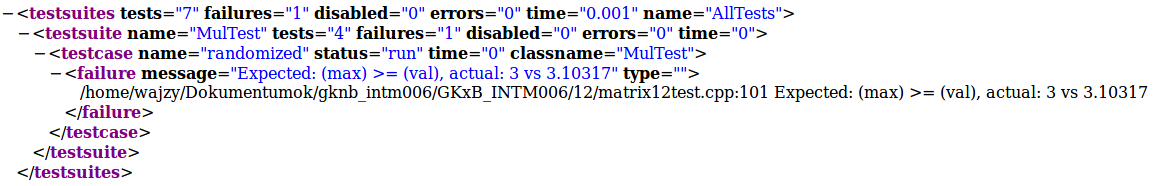
\includegraphics{./xmlout.png}}
  \end{block}
  \begin{itemize}
    \item Az XML megjeleníthető különféle eszközökkel, pl. %
\hiv{\href{https://wiki.jenkins.io/display/JENKINS/xUnit+Plugin}{Jenkins/xUnit}}-tal
  \end{itemize}
\end{frame}

\subsection{Kivételek és haláltesztek}

\begin{frame}
  Egészítsük ki a konstruktort kivétel dobásával, ha az eredeti vektor sorai nem azonos elemszámúak!
  \begin{exampleblock}{\textattachfile{13/matrix13.h}{13/matrix13.h} %
    (\textattachfile{13/CMakeLists.txt}{13/CMakeLists.txt})}
    \scriptsize
    \lstinputlisting[style=cpp,linerange={6-16},numbers=left,firstnumber=6]{13/matrix13.h}
    \lstinputlisting[style=cpp,linerange={26-26},numbers=left,firstnumber=26]{13/matrix13.h}
  \end{exampleblock}
\end{frame}

\begin{frame}
  \begin{exampleblock}{\textattachfile{13/matrix13.h}{13/matrix13.h}}
    \scriptsize
    \lstinputlisting[style=cpp,linerange={41-56},numbers=left,firstnumber=41]{13/matrix13.h}
  \end{exampleblock}
\end{frame}

\begin{frame}
  Módosítsuk és egészítsük ki tesztünket!
  \begin{exampleblock}{\textattachfile{13/matrix13test.cpp}{13/matrix13test.cpp}}
    \scriptsize
    \lstinputlisting[style=cpp,linerange={20-32},numbers=left,firstnumber=20]{13/matrix13test.cpp}
  \end{exampleblock}
\end{frame}

\begin{frame}
  \begin{exampleblock}{\textattachfile{13/matrix13test.cpp}{13/matrix13test.cpp}}
    \footnotesize
    \lstinputlisting[style=cpp,linerange={33-45},numbers=left,firstnumber=33]{13/matrix13test.cpp}
  \end{exampleblock}
\end{frame}

\begin{frame}
  \begin{exampleblock}{\textattachfile{13/matrix13test.cpp}{13/matrix13test.cpp}}
    \lstinputlisting[style=cpp,linerange={47-55},numbers=left,firstnumber=47]{13/matrix13test.cpp}
  \end{exampleblock}
\end{frame}

\begin{frame}
  \begin{center}
    Kivételek kiváltásával szemben támasztható követelmények
    \medskip\\
    \resizebox{\textwidth}{!}{
    \begin{tabular}{llp{0.3\textwidth}}
      \textbf{Végzetes hibákhoz} & \textbf{Nem végzetes hibákhoz} & \textbf{Követelmény}\\ \hline
      ASSERT\_THROW(\emph{statement}, \emph{exception\_type}); & EXPECT\_THROW(\emph{statement}, \emph{exception\_type}); & 
\emph{statement} hatására \emph{exception\_type} kivételnek kell keletkeznie \\
      ASSERT\_ANY\_THROW(\emph{statement}); & EXPECT\_ANY\_THROW(\emph{statement}); & \emph{statement} hatására 
valamilyen kivételnek kell keletkeznie \\
      ASSERT\_NO\_THROW(\emph{statement}); & EXPECT\_NO\_THROW(\emph{statement}); & \emph{statement} hatására 
semmilyen kivételnek sem szabad keletkeznie \\
    \end{tabular}
    }
  \end{center}
\end{frame}

\begin{frame}
  A haláltesztek (Death Tests) azt ellenőrzik, hogy valamilyen körülmény hatására a program leáll-e. Egészítsük ki a 
konstruktort úgy, hogy negatív sor- vagy oszlopszám esetén 1 hibakóddal álljon le a program!
  \begin{exampleblock}{\textattachfile{14/matrix14.h}{14/matrix14.h} %
    (\textattachfile{14/CMakeLists.txt}{14/CMakeLists.txt})}
    \small
    \lstinputlisting[style=cpp,linerange={28-33},numbers=left,firstnumber=28]{14/matrix14.h}
  \end{exampleblock}
\end{frame}

\begin{frame}
  Ellenőrizzük, hogy a program valóban leáll-e az elvárt módon!
  \begin{exampleblock}{\textattachfile{14/matrix14test.cpp}{14/matrix14test.cpp}}
    \small
    \lstinputlisting[style=cpp,linerange={119-123},numbers=left,firstnumber=119]{14/matrix14test.cpp}
  \end{exampleblock}
\end{frame}

\begin{frame}
  \begin{center}
    Halálteszteket támogató makrók
    \medskip\\
    \resizebox{\textwidth}{!}{
    \begin{tabular}{llp{0.3\textwidth}}
      \textbf{Végzetes hibákhoz} & \textbf{Nem végzetes hibákhoz} & \textbf{Követelmény}\\ \hline
      ASSERT\_DEATH(\emph{statement}, \emph{matcher}); & EXPECT\_DEATH(\emph{statement}, \emph{matcher}); & \emph{statement} 
programleállást idéz elő \emph{matcher} üzenettel \\
      ASSERT\_DEATH\_IF\_SUPPORTED(\emph{statement}, \emph{matcher}); & EXPECT\_DEATH\_IF\_SUPPORTED(\emph{statement}, 
\emph{matcher}); & Csak akkor ellenőrzi, hogy \emph{statement} 
programleállást idéz-e elő \emph{matcher} üzenettel, ha a haláltesztek támogatottak \\
      ASSERT\_EXIT(\emph{statement}, \emph{predicate}, \emph{matcher}); & EXPECT\_EXIT(\emph{statement}, \emph{predicate}, 
\emph{matcher}); & \emph{statement} 
programleállást idéz elő \emph{matcher} üzenettel, a kilépési kódot \emph{matcher}-re állítja \\
    \end{tabular}
    }
  \end{center}
\end{frame}

\begin{frame}
  Paraméterezés:
  \begin{description}[mm]
    \item[\emph{statement}] \hfill\\ A programleálláshoz vezető (egyszerű vagy összetett) utasítás.
    \item[\emph{predicate}] \hfill\\ Függvény vagy függvény objektum, ami \texttt{int} paramétert vár és \texttt{bool}-t 
szolgáltat:
    \begin{itemize}
      \item \texttt{::testing::ExitedWithCode(exit\_code)} \\ Az elvárt kilépési kódot ellenőrzi.
      \item \texttt{::testing::KilledBySignal(signal\_number)} \\ Ellenőrzi, hogy a programot az elvárt jelzés szakította-e 
félbe (Windows-on nem támogatott).
    \end{itemize}
  \end{description}
\end{frame}

\begin{frame}
  Paraméterezés folyt.:
  \begin{description}[mm]
    \item[\emph{matcher}] \hfill\\ A szabvány hibacsatornára írt, elvárt üzenet. Ellenőrizhető:
    \begin{enumerate}
      \item 
\hiv{\href%
{https://github.com/google/googletest/blob/master/googlemock/docs/cook\_book.md\#using-matchers-in-googletest-assertions}%
{GMock illesztővel}} (\emph{const std::string\&}-t illeszt)
      \item 
\hiv{\href{http://pubs.opengroup.org/onlinepubs/009695399/basedefs/xbd_chap09.html\#tag\_09\_04}%
{Perl-kompatibilis}} \hiv{\href{https://en.wikipedia.org/wiki/Regular_expression\#POSIX\_basic\_and\_extended}%
{reguláris kifejezéssel}} (A ,,csupasz'' karakterláncokat \texttt{ContainsRegex(str)}-rel értékelik ki.)
    \end{enumerate}
  \end{description}
  Megjegyzések
  \begin{itemize}
    \item A 0 kilépési kóddal leálló programot nem tekintik ,,halott'' programnak. A leállítás általában 
\texttt{abort()}, \texttt{exit()} hívással vagy egy jelzéssel történik.
    \item A haláltesztek készletének neve \texttt{DeathTest}-re kell, hogy végződjön 
(\hiv{\href{https://github.com/google/googletest/blob/master/googletest/docs/advanced.md\#death-tests-and-threads}{részletek}}). 
Szálbiztos környezet szükséges lehet.
  \end{itemize}
\end{frame}


% Integráció IDE-kkel

\section{Források}

\begin{frame}
  Tesztelésről általában\\
  \hiv{\href{https://www.tankonyvtar.hu/hu/tartalom/tamop425/0046\_szoftverteszteles/index.html}%
  {Ficsor Lajos, Kovács László, Kusper Gábor, Krizsán Zoltán: Szoftvertesztelés}}\\
  \hiv{\href{https://hstqb.org/downloadarea/istqb-ctfl-syllabus-2018-magyar/}{ISTQB CTFL Syllabus 2018}}\\
  \hiv{\href{https://glossary.istqb.org/en/search/}{Szakkifejezések kereshető gyűjteménye}}\\
  \vfill
  googletest\\
  \hiv{\href{https://github.com/google/googletest/blob/master/googletest/docs/primer.md}%
    {Hivatalos Google tutorial, bevezető}}\\
  \hiv{\href{https://github.com/google/googletest/blob/master/googletest/docs/advanced.md}%
    {Hivatalos Google tutorial, fejlett technikák}}\\
  \hiv{\href{https://github.com/google/googletest/blob/master/googletest/docs/faq.md}{googletest FAQ}}\\
  \hiv{\href{https://www.eriksmistad.no/getting-started-with-google-test-on-ubuntu/}%
    {Ubuntu-specifikus részletek}}\\
  \hiv{\href{https://developer.ibm.com/articles/au-googletestingframework/}{IBM tananyag a googletest-hez}}\\
\end{frame}

\end{document}
